\chapter{INTRODUCTION}




\section{Motivation}
Currently the main channel for job seekers are online job finding web sites, like indeed or  monster etc, that make the job finding process easier and decrease the recruitment time. But most such web sites only allow users to use key word to search the jobs, which makes job searching as tedious and blind task. For example, I used keyword ``Java'' to search jobs with location restriction Mountain View, CA on the job searching site indeed.com, the web site returned about 7,000 jobs (Figure~\ref{fig:Indeed}). The number of results of job searching is huge but un-ranked, so the job seeker has to review every job description. Since no one has enough time to read all the jobs in the searching result, the actual quality of job searching service is low. This is a classic problem of information overflow.


\begin{figure}[htbp]
  \centering
  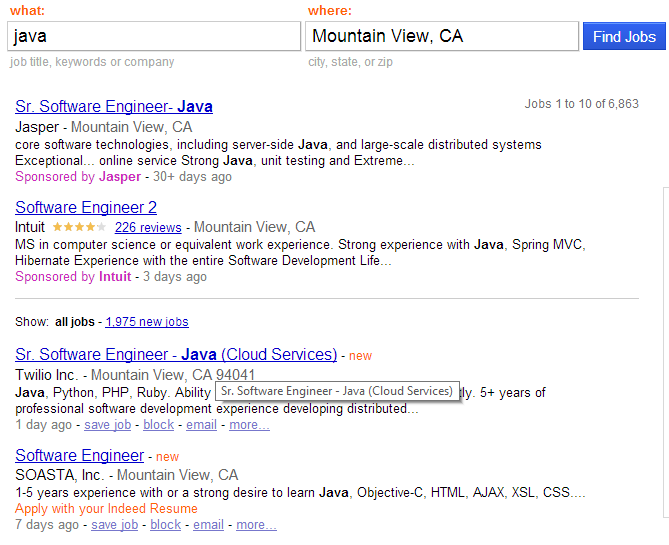
\includegraphics[scale=0.4]{images/indeed1.png}
  \caption{Search result of Indeed}
  \label{fig:Indeed}
\end{figure}

The reason for such result is because current job searching web sites use the same information retrieval technology like ``Inverted index'' \cite{zobel2006inverted} as the common search engines, which just use keywords to map all the stored documents. Modern search engines all have some ranking algorithms to sort the searching result, like page rank \cite{page1999pagerank}, so the top results always be the most related ones. But such algorithms are unavailable to the job searching systems, because the criteria  of how to rank the job searching result is very personalized. A great job opening for one job seeker maybe looks not good to the other, because the goodness of a job to a specular job seeker is heavily depend on his personal background, like his education or professional experience etc.

Since the people's resumes contain the most important background information, we believe the content of the resume could be used to rank the job openings. In this thesis we created a web system which could use the resumes of job seekers to find the jobs that match their profiles best. The main idea is to calculate the similarity between the candidate model and job models, which should be generated from resumes and job descriptions. I want to transfer the job searching task from key word searching to candidate model matching. The matching result should be sorted by the matching score, higher matching score means a better matching. The matching algorithm not only help job seekers to find the appreciate job opening, but also offer priority to them.~\cite{gueutal2006brave}  The job with higher matching score means the job is more appropriate to the job seeker, and if he applies the job, the chance of getting the interview will be higher as well. Figure~\ref{fig:Matching} shows how this approach works.


\begin{figure}[htbp]
  \centering
  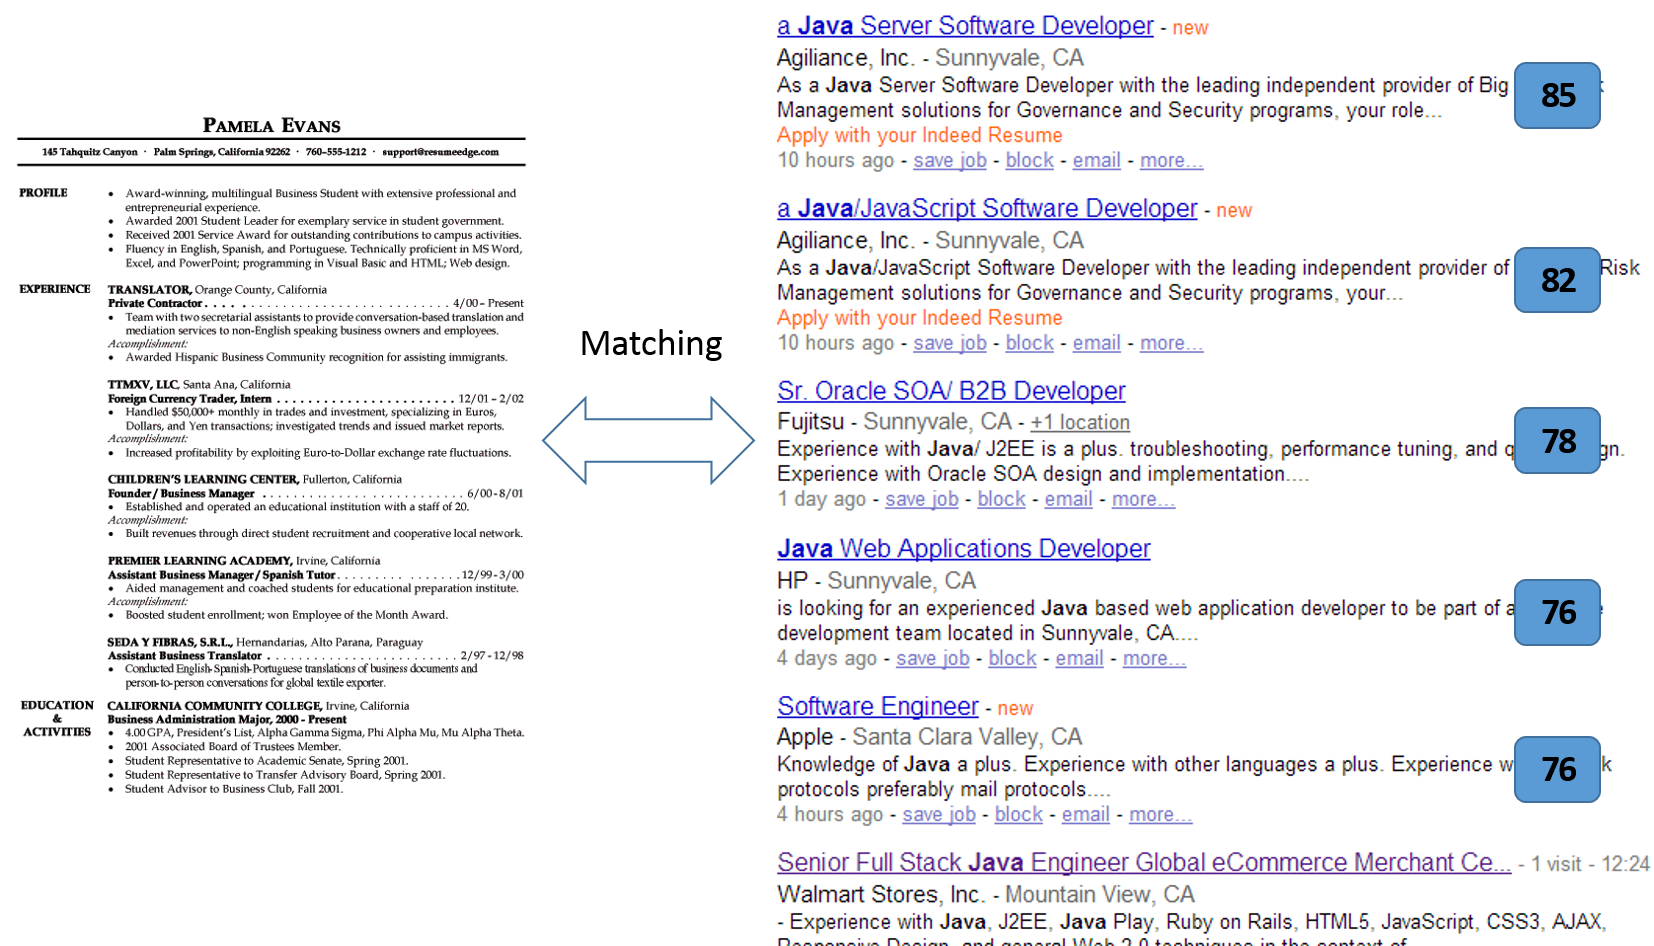
\includegraphics[scale=0.5]{images/matching.png}
  \caption{Matching the job opening with Resume}
  \label{fig:Matching}
\end{figure}

\section{Contribution}

We make the following contributions in this work:

\begin{enumerate}
    \item  We created a finite automata based matching tool to extract information from unstructured data source.
    \item  We created a domain specific Ontology for recruitment.
    \item  We proposed statistical based Ontology similarity measure.
    \item  We proposed a approach which combine the keyword searching method and model matching to retrieval jobs.
\end{enumerate}

\section{Organizations}
The subsequent chapters are organized as follows: We first describe what has been done in terms of prior work.  We introduce some basic conception of recommender systems, and how to apply recommender technologies into Job Recommender Systems. Some previous Job Recommender Systems will be introduced,  their advantages and limits will be discussed as well.  Two import problems of content-based Job Recommender Systems, Information Extraction and Similarity Calculation, will be fully introduced.

Then we introduce the JobFinder, the Personalized Resume-Job Matching System. At first we give a overview of the system, include architecture and interface. Then we explained details of how we resolve the problems of information extraction and model similarity between job resumes and resumes. We proposed a finite state transducer tool which matches patterns in sentence, and extracts related information. Ontology play an important role in this system. We will present how to construct the domain specific Ontology. We also give a brief review of different Ontology similarity measures. We proposed a statistical-based Ontology Similarity measure. 

Finally, we evaluate our information extraction approach, and accuracy of ontology similarity. To evaluate the performance of the system  we compared our algorithm to some classical information retrieval approaches by precision@k and NDCG. We created a data set of 100 job descriptions as documents, and use resumes as query to retrieval documents. The result shows the ranking performance is improved. 
